\documentclass[../HFT-main.tex]{subfiles} 

%\title{The I Know That You Know That I Know Protocol} %} TIKTYKTIK} Need to get \TIK Macro in this

%\author{Alan Karp}
%\date{\today}

\definecolor{red}{rgb}{0.6, 0, 0} % RGB values for dark red


\begin{document}
%\maketitle

\clearpage
\section{TIKTYKTIK Details} 

 \marginnote{
 \begin{framed} 
 \noindent  \textbf{NOTE TO READER}\\
 THIS FORMAT IS DESIGNED FOR YOU TO ADD  COMMENTS AND QUESTIONS IN THE RIGHT MARGIN, ETHER IN YOUR FAVORITE PDF VIEWER, OR IN THE LATEX DOCUMENT
 \end{framed}}
%Alan Karp

TIKTYKTIK is like the alternating-bit and stop-and-wait protocols in that receipt of a
packet over a link is acknowledged over that link with a “signal” packet. 
In that sense,
these three protocols implement credit based flow control, which simplifies buffer management and makes it possible to not have to drop packets when there is a lot of traffic.

TIKTYKTIK adds a second round trip, which provides partial common knowledge
helpful for recovery from link failures. This document walks through TIKTYKTIK
showing how that common knowledge is used.
First look at the various stages of common knowledge as the protocol runs without
failure when Alice sends a packet to Bob.

\begin{enumerate}
\item Alice sends the packet to Bob
	\begin{itemize}
	\item Alice doesn’t know if Bob received the packet
	\item Bob does not know the packet exists
	\end{itemize}
\item Bob receives the packet
	\begin{itemize}
	\item Bob knows that Alice doesn’t know that Bob received the packet
	\end{itemize}
\item Bob sends a signal to Alice
	\begin{itemize}
	\item Bob doesn’t know if Alice knows that Bob received the packet
	\end{itemize}
\item Alice receives the signal
	\begin{itemize}
	\item Alice knows that Bob received the packet
	\item Alice knows that Bob doesn’t know that Alice knows that Bob received the
packet
	\end{itemize}
\item Alice sends the signal
	\begin{itemize}
	\item Alice doesn’t know if Bob knows that Alice knows that Bob received the
packet.
	\end{itemize}
\item Bob receives the signal
	\begin{itemize}
	\item Bob knows that Alice knows that Bob received the packet.
	\item Bob doesn’t know if Alice knows that Bob knows that Alice knows that Bob
received the packet.
	\item Bob can forward the packet
	\end{itemize}
\item Alice receives the signal
	\begin{itemize}
	\item Alice knows that Bob knows that Alice knows that Bob received the packet.
	\item Alice can delete her copy of the packet.
	\end{itemize}
\end{enumerate}

This common knowledge is not needed if links never fail. Alice could delete the packet
as soon as she sent it, and Bob could forward it as soon as he received it. That’s what
current systems do and why it’s so hard to recover from a link failure.

A data packet can serve as a signal.\sidenote{A data packet can serve as a signal.}
Links can fail in a number of ways. If they physically break or are unplugged, the PHY
detects the lost of electrical signal and informs the higher layers. Links can also fail
silently, such as when the NIC misbehaves. They can also fail in one direction but not
the other. Silent failures can be detected in these protocols because a signal will never
be received in either direction. In that sense, there is a level of common knowledge on
a link failure.
In what follows, I’ll describe what happens when Alice wants to send a packet to Bob,
but the link fails at various steps of the protocol. The link is no longer used once one of
these failures occurs. (The link can be used later after re-initializing the connection.)

\begin{itemize}
    \item 1  Alice has a packet to send when link fails
    \begin{itemize}
        \item Alice
        \begin{itemize}
            \item Knows Bob doesn’t have the packet
            \item Knows Alice is responsible for it
        \end{itemize}
        \item Bob
        \begin{itemize}
            \item Doesn’t know the packet exists
        \end{itemize}
    \end{itemize}
    
    \item 2 Alice sends the packet to Bob then link fails
    \begin{itemize}
        \item Alice
        \begin{itemize}
            \item Doesn’t know if Bob got the packet
            \item Knows that Bob knows Alice is responsible
        \end{itemize}
        \item Bob
        \begin{itemize}
            \item Doesn’t know that the packet exists
        \end{itemize}
    \end{itemize}

    \item  3 Bob receives the packet then link fails
    \begin{itemize}
        \item Bob
        \begin{itemize}
            \item Knows that Alice knows that Alice is responsible
        \end{itemize}
        \item Alice
        \begin{itemize}
            \item \textcolor{red}{Alice doesn’t know if Alice or Bob is responsible}
        \end{itemize}
    \end{itemize}

    \item 4 Bob sends signal then link fails
    \begin{itemize}
        \item Bob
        \begin{itemize}
            \item {Doesn’t know if Alice got the signal}
            \item \textcolor{red}{Doesn’t know if Bob or Alice is responsible}
        \end{itemize}
        \item Alice
        \begin{itemize}
            \item \textcolor{red}{Alice doesn’t know if Alice or Bob is responsible}
        \end{itemize}
    \end{itemize}

    \item 5 Alice receives the signal then link fails
    \begin{itemize}
        \item Alice
        \begin{itemize}
            \item Knows that Bob is responsible
            \item Knows that Bob doesn’t know he is responsible
        \end{itemize}
        \item Bob
        \begin{itemize}
            \item Doesn’t know if Alice got the signal
            \item \textcolor{red}{Doesn’t know if Alice knows that Bob is responsible}
        \end{itemize}
    \end{itemize}

    \item 6 Alice sends signal then link fails
    \begin{itemize}
        \item Alice
        \begin{itemize}
            \item Knows that Bob is responsible
            \item \textcolor{red}{Doesn’t know if Bob knows he is responsible}
        \end{itemize}
        \item Bob
        \begin{itemize}
            \item \textcolor{red}{Doesn’t know if he’s responsible for the packet}
        \end{itemize}
    \end{itemize}

    \item 7 Bob receives the signal then link fails
    \begin{itemize}
        \item Bob
        \begin{itemize}
            \item Knows that Alice knows that Bob is responsible
        \end{itemize}
        \item Alice
        \begin{itemize}
            \item Doesn’t know if Bob knows that Bob is responsible
        \end{itemize}
    \end{itemize}

    \item 8 Bob sends signal then link fails
    \begin{itemize}
        \item Bob
        \begin{itemize}
            \item Knows that he is responsible
            \item Doesn’t know if Alice knows he is responsible
        \end{itemize}
        \item Alice
        \begin{itemize}
            \item Knows that Bob is responsible
            \item Doesn’t know if Bob knows that Bob is responsible
        \end{itemize}
    \end{itemize}

    \item 9 Alice receives signal
    \begin{itemize}
        \item Alice
        \begin{itemize}
            \item Knows that Bob knows that he is responsible
        \end{itemize}
    \end{itemize}
\end{itemize}

At this point, Alice knows that Bob knows that Bob is responsible, and Bob knows that
Alice knows that Bob is responsible.

The items in \textcolor{red}{red} indicate where incomplete common knowledge needs to be resolved
over the new path between Alice and Bob.

%\end{document}

\newpage
\section{Feedback from ChatGPT}

The analysis you provided explores how "common knowledge" operates within the TIKTYKTIK protocol, especially in the context of link failure recovery. The progression of common knowledge is explained through several stages, starting with Alice sending a packet to Bob and progressing through various acknowledgment signals and link failures.

\subsection{Key observations:}

\begin{enumerate}
\item Common Knowledge Phases: The stages you outlined show how knowledge evolves between Alice and Bob as they interact, especially when there’s uncertainty about packet receipt and acknowledgment. These stages are useful for understanding how communication protocols can handle and resolve ambiguities.

\item Link Failures: You go into detail about different link failure scenarios, from Alice sending the packet before failure to Bob acknowledging receipt of the packet after a failure. Each failure step indicates the differing levels of knowledge held by Alice and Bob. These steps, especially when the link fails, highlight the challenges of network fault tolerance, and the importance of "common knowledge" for recovering from these failures.

\item Protocol Behavior with Failure: The distinction between knowledge of responsibility and knowledge of receipt is well captured. The incomplete common knowledge as the link fails suggests that TIKTYKTIK, by adding a second round-trip acknowledgment, resolves uncertainties that could otherwise hinder recovery.

\end{enumerate}

\subsection{Suggested Refinements:}

\begin{description}
	\item [Clarity:] Consider rephrasing the stages of knowledge with more emphasis on the protocol mechanics and timing of messages. It could be helpful to lay out the flow of the protocol in a diagram or a clearer timeline to illustrate the evolution of knowledge.
	\item [Link Failures and Recovery:] While the failure scenarios are well outlined, you could further enhance the analysis by providing examples of real-world failure cases and how TIKTYKTIK compares to other protocols in handling these failures. For example, you could contrast how TCP handles packet loss versus how TIKTYKTIK’s multi-step acknowledgment approach helps resolve knowledge gaps.
	\item [Mathematical Notation:]If possible, you could introduce formal mathematical notations to express the knowledge states. This would help readers better grasp the protocol’s behavior in a more structured form.
\end{description}

%Would you like to expand or refine any specific section, or perhaps work on the failure recovery flow with more technical detail?

%\newpage
%
%\begin{marginfigure}
%  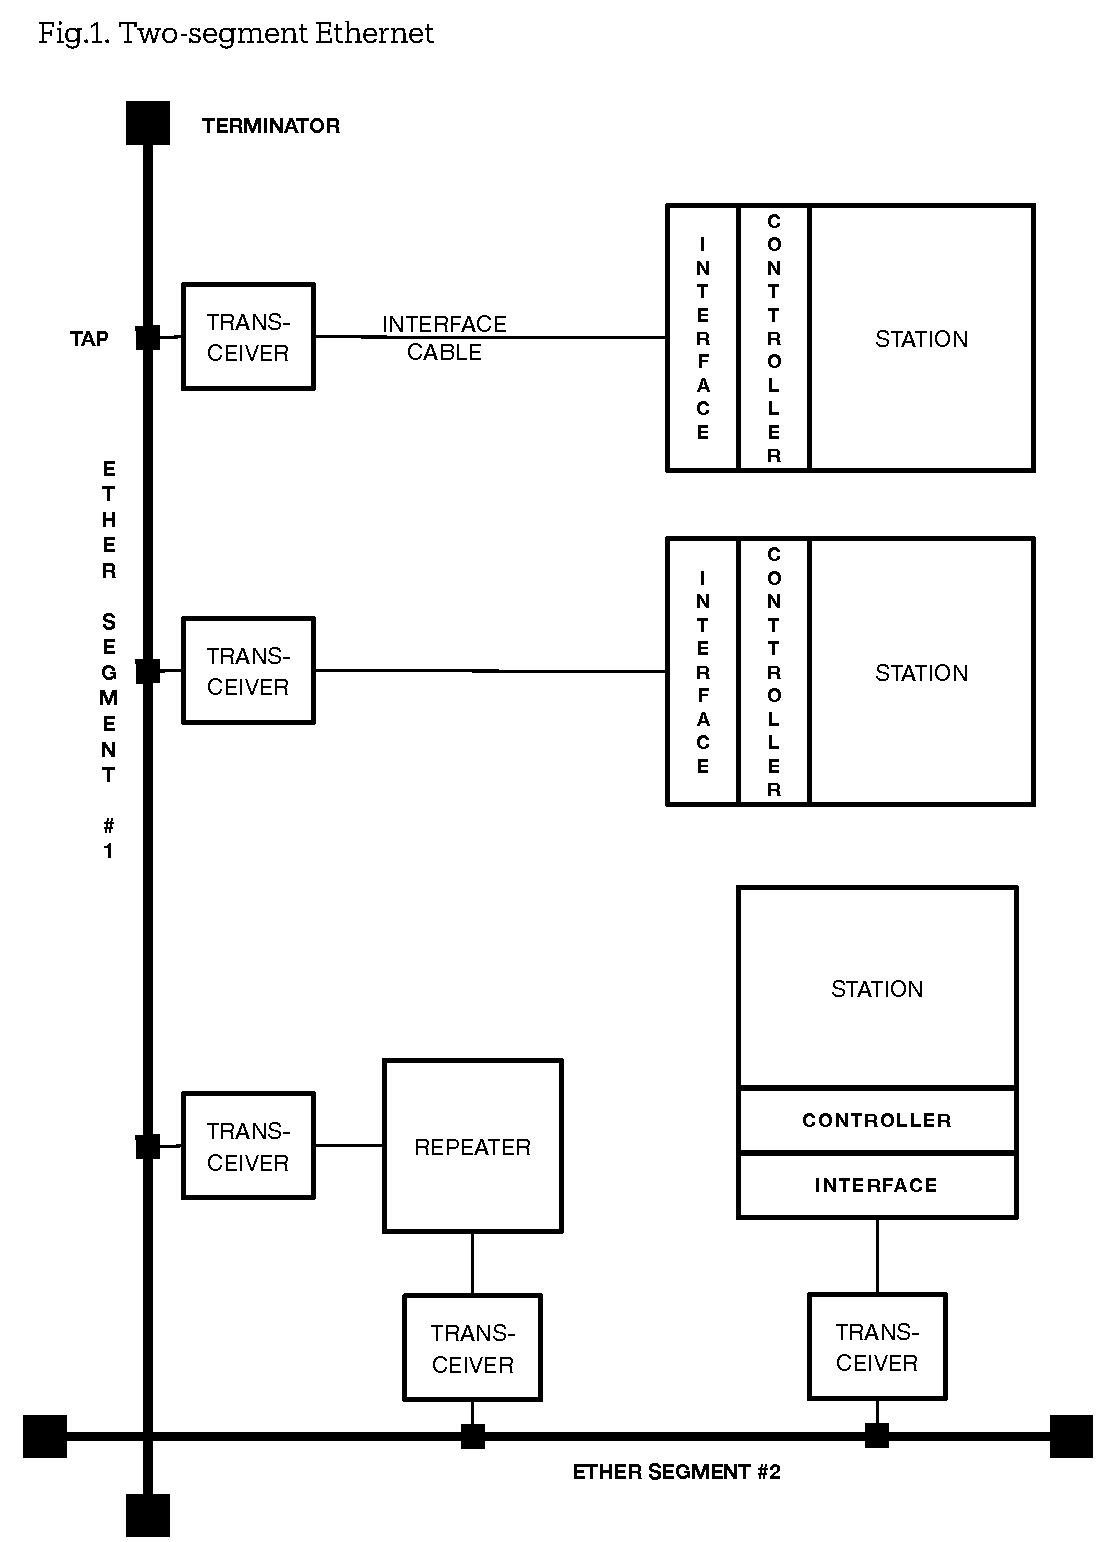
\includegraphics[width=\linewidth]{../../FIGURES/Omni-Figure-1.pdf}
%  \caption{Original Ethernet Repeater )}
%  \vspace{25pt}
%\end{marginfigure}
%
%
%\begin{marginfigure}
%  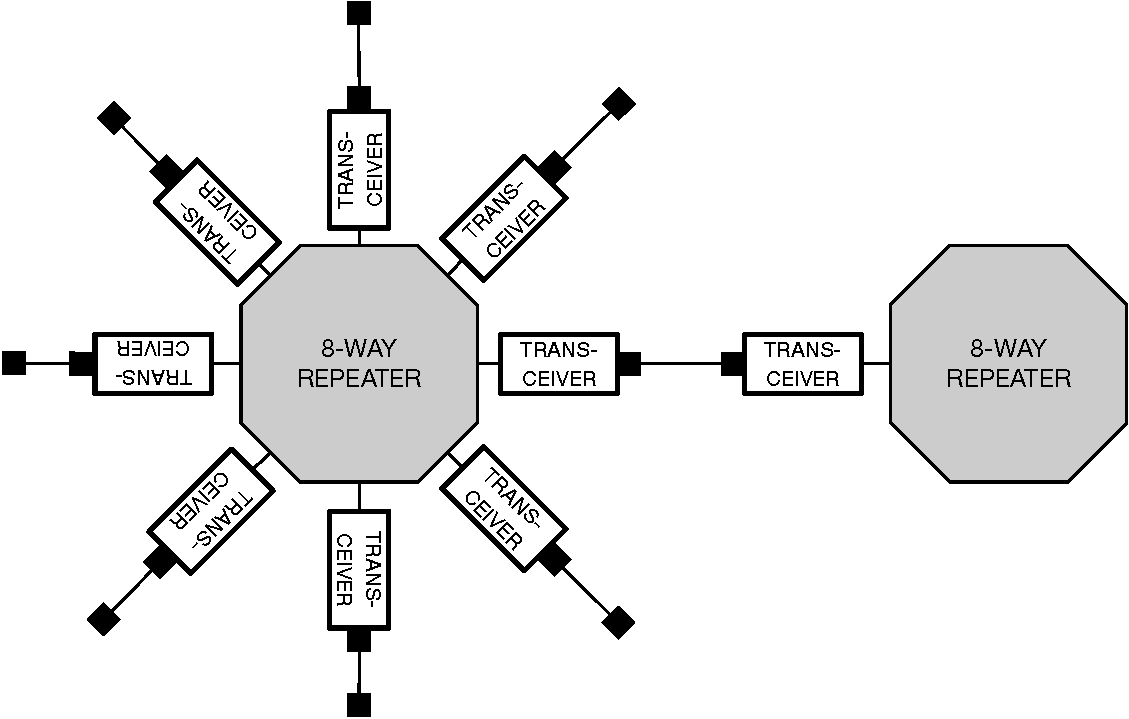
\includegraphics[width=\linewidth]{../../FIGURES/8-way-repeater.pdf}
%  \caption{Original Ethernet Repeater extended from valency-2 to valency-8)}
%\end{marginfigure}
%
%
%\section{Bob Metcalfe}
%
%\begin{itemize}
%\item “The Parc Ethernet was Manchester, but not high voltage alternating with low voltage. The cable was not driven or driven, on or off, leaving the cable off/undriven half the time, so that collisions could be detected. Half the time during a packet the cable would be undriven. Clock was recovered from transitions to or from driven state in the middle of each bit cell.”
%
%\item “I remember waking up, screaming in the night, terrified we couldn’t get our transceivers under 4 picofarads”
%
%\item “Wondering if some sort of BACKOFF THEORY would be deep enough for a talk at Ethernet’s 50th and the SmartNIC keynote and …”
%
%\item “Ethernet doesn’t work in Theory, it only works in Practice”
%
%\item “Close the Loop”
%\end{itemize}



\end{document}